\section{Introduction}

Suppose that you been offered the opportunity to invest in the Volatile Chemical Corporation. Like the chemicals the company produces, the stock price of the Volatile Chemical Corporation is rather volatile. You are allowed to buy one unit of stock only one time and then sell it at a later date, buying and selling after the close of trading for the day. To compensate for this restriction, you are allowed to learn what the price of the stock will be in the future. Your goal is to maximize your profit. Figure 1 shows the price of the stock over a 17-day period. You may buy the stock at any one time, starting after day 0, when the price is 100 dollars per share. Of course, you would want to "buy low, sell high" buy at the lowest possible price and later on sell at the highest possible price to maximize your profit. Unfortunately, you might not be able to buy at the lowest price and then sell at the highest price within a given period. In Figure 1, the lowest price occurs after day 7, which occurs after the highest price, after day 1.
You might think that you can always maximize profit by either buying at the lowest price or selling at the highest price. For example, in Figure 1, we would maximize profit by buying at the lowest price, after day 7. If this strategy always worked, then it would be easy to determine how to maximize profit: find the highest and lowest prices, and then work left from the highest price to find the lowest prior price, work right from the lowest price to find the highest later price, and take the pair with the greater difference. Figure 2 shows a simple counterexample demonstrating that the maximum profit sometimes comes neither by buying at the lowest price nor by selling at the highest price. \hfill \break

\begin{figure}[H]
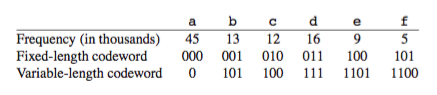
\includegraphics[width = 16.5cm, height = 5cm]{1.png}
\centering \linebreak \linebreak Figure 1: {\small Information about the price of stock in the Volatile Chemical Corporation after the close of trading over a period of 17 days. The horizontal axis of the chart indicates the day, and the vertical axis shows the price. The bottom row of the table gives the change in price from the previous day.}
\end{figure}

\begin{figure}[H]

\includegraphics[width = 16.5cm, height = 5cm]{2.png}
\centering \linebreak \linebreak Figure 2: {\small An example showing that the maximum profit does not always start at the lowest price or end at the highest price. Again, the horizontal axis indicates the day, and the vertical axis shows the price. Here, the maximum profit of 3 dollars per share would be earned by buying after day 2 and selling after day 3. The price of 7 dollars after day 2 is not the lowest price overall, and the price of 10 dollars after day 3 is not the highest price overall.}
\end{figure} \hfill

\pagebreak